%!TEX program = xelatex
\documentclass[tikz, border=5pt]{standalone}
\usepackage{pgfplots}
\usepackage{xcolor}
\usepgfplotslibrary{patchplots, colormaps, colorbrewer}
\pgfplotsset{compat=1.18}

\begin{document}
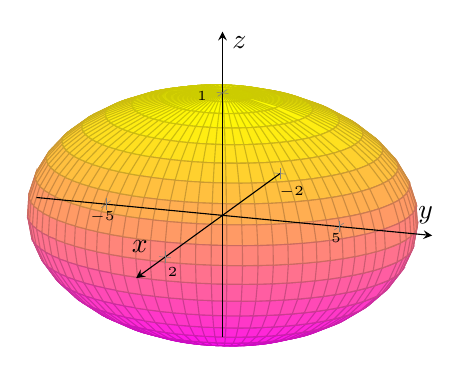
\begin{tikzpicture}
    \begin{axis}[
        view={110}{20},
        axis lines=center,
        xlabel=$x$, ylabel=$y$, zlabel=$z$,
        xmax=3, ymax=9, zmax=1.5,  % 根据新参数调整坐标范围
        tick label style={font=\tiny},
        axis on top
    ]
        \addplot3 [
            colormap/spring,
            surf,
            z buffer=sort,
            samples=40,  % 调整采样率
            domain=0:2*pi,  % 新参数域
            y domain=0:2*pi
        ] (
            {2*sin(deg(x))*cos(deg(y))},  % 椭球面参数方程
            {8*sin(deg(x))*sin(deg(y))},
            {1*cos(deg(x))}
        );
    \end{axis}
\end{tikzpicture}
\end{document}